\subsection{相補フィルタと共分散で表す残差不確かさ}

差動二輪ロボットや小型姿勢実験で IMU を使うと、最初に観測される限界は二つに分かれる。ジャイロの角速度は短い時間では滑らかで、ロボットが加速しても重力以外の力を直接は角度に混ぜない。しかし、角速度に小さなバイアスが含まれると、積分した角度はゆっくり片側へ流れていく。一方、加速度計から作る傾きは、静止に近いときには重力方向から絶対的な角度を与えるが、並進加速度や振動がある区間では、重力ではない加速度まで傾きとして解釈してしまう。したがって、ジャイロだけでは低周波のドリフトが残り、加速度計だけでは高周波のノイズと加速時の外乱が残る。

ここでは、一軸の小さな傾き $\theta$ を対象にする。サンプリング周期を $\Delta t$、ジャイロ測定を $\omega_{m,k}$、加速度計から作った傾き測定を $\theta_{\mathrm{acc},k}$ と置く。測定の典型的な近似は
\begin{align}
  \omega_{m,k}
  &=\dot{\theta}_k+b_k+n_{g,k},\\
  \theta_{\mathrm{acc},k}
  &=\theta_k+n_{a,k}+d_{a,k}
\end{align}
である。$b_k$ はゆっくり変化するジャイロバイアス、$n_{g,k}$ と $n_{a,k}$ は零平均の測定ノイズ、$d_{a,k}$ は並進加速度や振動によって加速度計の傾き換算へ混ざる成分である。ジャイロだけで
\begin{equation}
  \hat{\theta}^{g}_k
  =
  \hat{\theta}^{g}_{k-1}+\omega_{m,k}\Delta t
\end{equation}
と積分すると、$b_k$ の和が角度へ蓄積する。反対に $\theta_{\mathrm{acc},k}$ をそのまま使うと、$n_{a,k}$ と $d_{a,k}$ が直接角度推定へ入る。図\ref{fig:flow6-complementary-covariance-examples}は、この二つの失敗を同じ時系列に置き、固定相補フィルタがどこまで修正し、どの不確かさを残すかを示している。

\begin{figure}[tb]
  \centering
  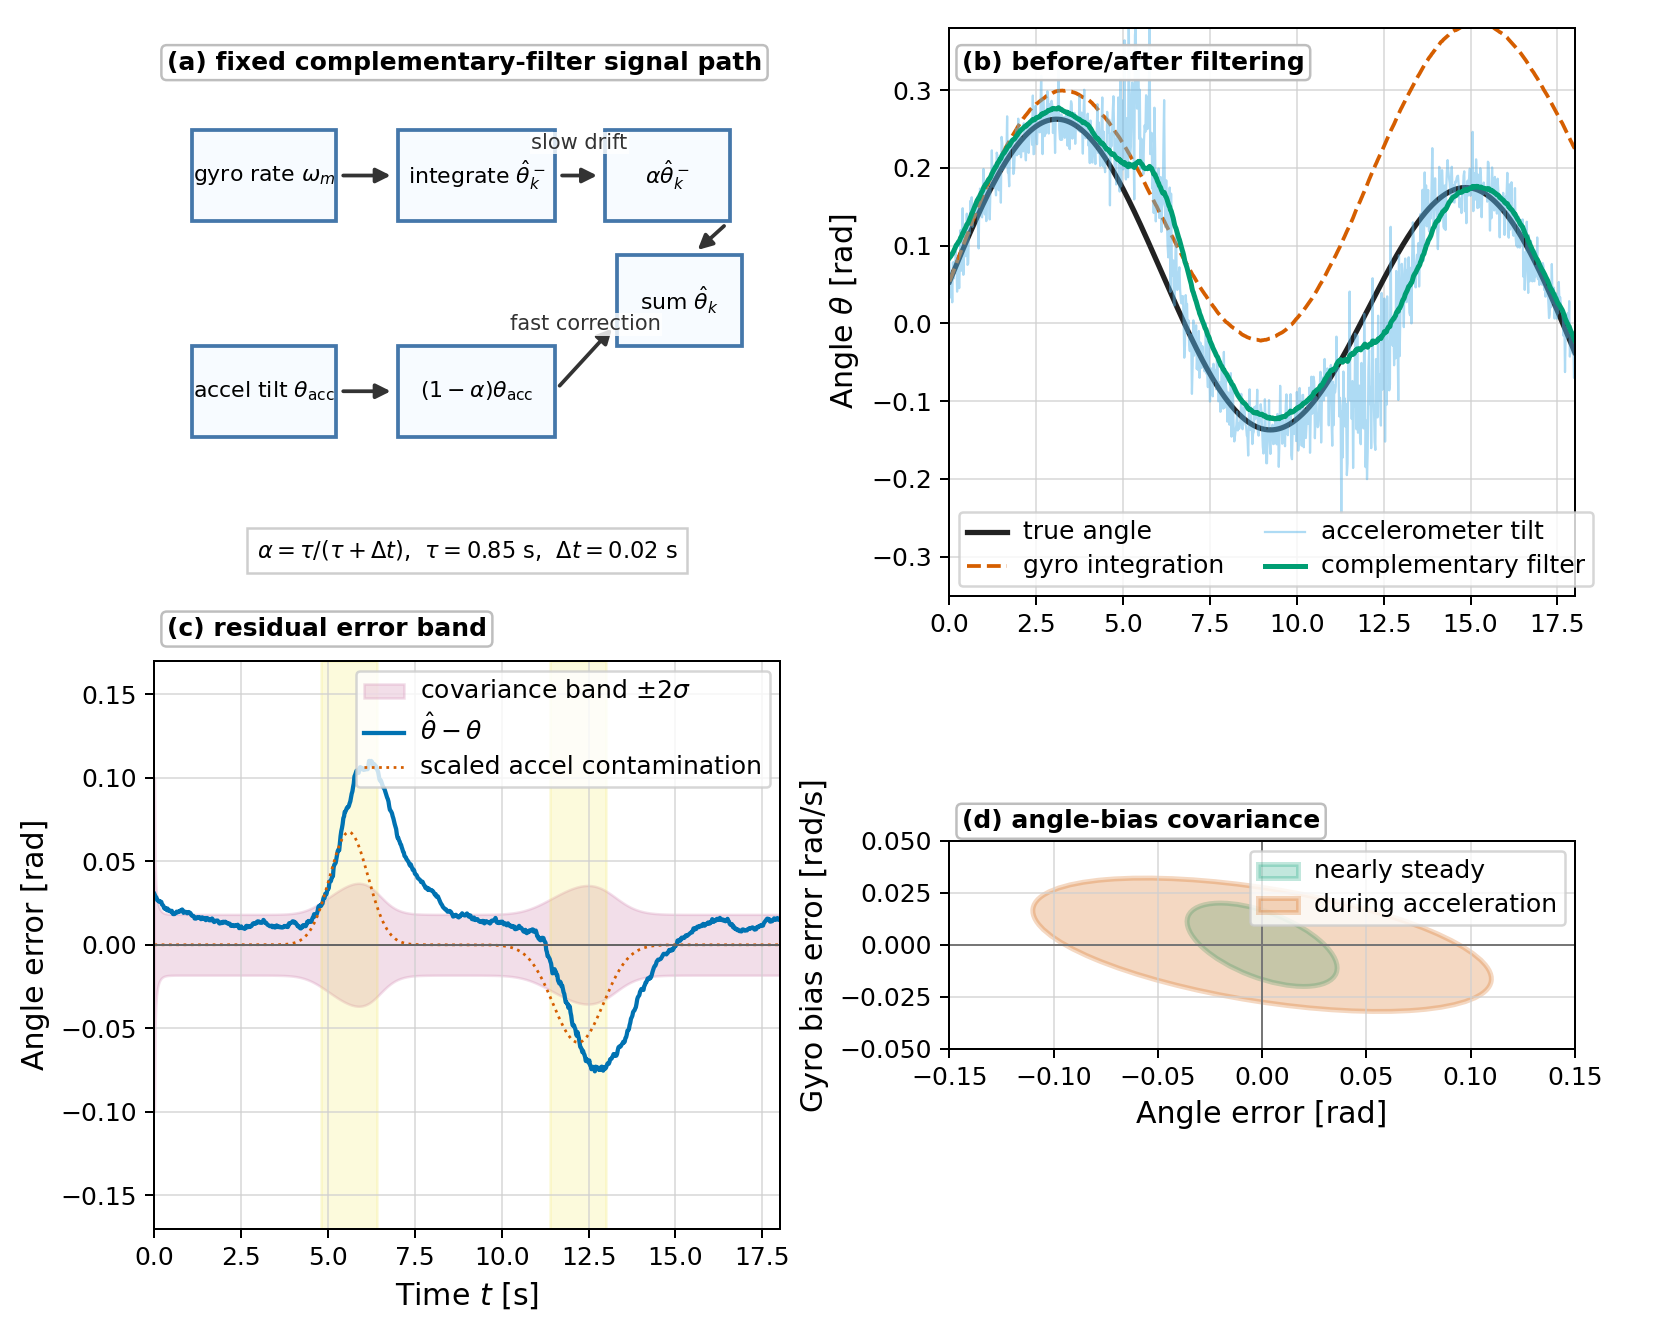
\includegraphics[width=0.98\linewidth]{figures/flow6_complementary_covariance_examples.png}
  \caption{ジャイロ積分、加速度計傾き、相補フィルタ、残差不確かさの関係。左上は固定係数の信号経路、右上はドリフトと加速度外乱を含む測定の前後比較、左下はフィルタ後の残差と共分散帯、右下は角度誤差とジャイロバイアス誤差の楕円表示である。加速区間では加速度計の見かけの傾きが悪化し、固定係数のままでは信頼度の変化を推定器の内部状態として保持できない。}
  \label{fig:flow6-complementary-covariance-examples}
\end{figure}

相補フィルタは、ジャイロ積分の低周波ドリフトと、加速度計傾きの高周波ノイズを互いに補わせる固定ゲインの推定器として書ける。連続時間で
\begin{equation}
  \dot{\hat{\theta}}
  =
  \omega_m+\frac{1}{\tau}
  \left(\theta_{\mathrm{acc}}-\hat{\theta}\right)
\end{equation}
と置くと、$\omega_m$ で角度を進めながら、時定数 $\tau$ で加速度計の傾きへ戻す一次遅れの補正になっている。この式を、補正項だけ後退 Euler で離散化すると
\begin{align}
  \hat{\theta}_k
  &=
  \hat{\theta}_{k-1}+\omega_{m,k}\Delta t
  +\frac{\Delta t}{\tau}
  \left(\theta_{\mathrm{acc},k}-\hat{\theta}_k\right),\\
  \left(1+\frac{\Delta t}{\tau}\right)\hat{\theta}_k
  &=
  \hat{\theta}_{k-1}+\omega_{m,k}\Delta t
  +\frac{\Delta t}{\tau}\theta_{\mathrm{acc},k},\\
  \hat{\theta}_k
  &=
  \alpha
  \left(\hat{\theta}_{k-1}+\omega_{m,k}\Delta t\right)
  +(1-\alpha)\theta_{\mathrm{acc},k}
\end{align}
を得る。ただし、この離散化では
\begin{equation}
  \alpha=\frac{\tau}{\tau+\Delta t},
  \qquad
  1-\alpha=\frac{\Delta t}{\tau+\Delta t}
\end{equation}
である。$\tau$ を大きくすると $\alpha$ は 1 に近づき、ジャイロ積分を長く信じるため、加速度計ノイズは入りにくいがドリフトの戻りは遅くなる。$\tau$ を小さくすると加速度計の補正は速くなるが、加速中の $d_{a,k}$ も角度推定へ入りやすい。図の例では $\Delta t=0.02\,\mathrm{s}$、$\tau=0.85\,\mathrm{s}$ なので $\alpha\simeq0.977$ であり、数十サンプルにわたってジャイロ側を主に使いながら、長い時間では加速度計側へ戻している。

この固定係数の形は、加速度計の信頼度が時間でほとんど変わらない区間では有効である。ところが、ロボットが急加速する区間では $\theta_{\mathrm{acc},k}$ の分散だけでなく、$d_{a,k}$ のような偏った誤差も増える。静止に近い区間では加速度計をもっと強く使いたくなり、加速区間では一時的に弱く使いたくなる。固定した $\alpha$ は、この信頼度の変化を状態として持たないため、図の残差のように、ドリフトが減ったあとにも加速区間のずれが残る。

この残ったずれを「どちらの測定をどの比率で使うか」という係数だけで扱う代わりに、推定誤差の分散として持つと、次の段階の設計量を定義できる。予測直後の角度不確かさを $P^-_k$、加速度計傾きの測定分散を $R_{\mathrm{acc},k}$ と置く。固定相補フィルタの係数をそのまま使うなら、独立な誤差を仮定した角度分散は近似的に
\begin{equation}
  P_k
  \simeq
  \alpha^2 P^-_k+(1-\alpha)^2R_{\mathrm{acc},k}
\end{equation}
で更新される。この式は、図の共分散帯のように「この時刻の推定値がどの程度広がりを持つか」を表す。しかし、係数 $\alpha$ 自体はまだ変わらないため、$R_{\mathrm{acc},k}$ が急に大きくなっても、測定を取り込む比率は同じままである。

測定の信頼度に応じて重みを変えるには、予測と測定の分散比からゲインを決める。一次元で書けば、ジャイロで進めた予測値を
\begin{equation}
  \theta^-_k
  =
  \hat{\theta}_{k-1}+\omega_{m,k}\Delta t
\end{equation}
とし、補正を
\begin{align}
  \hat{\theta}_k
  &=
  \theta^-_k
  +K_k\left(\theta_{\mathrm{acc},k}-\theta^-_k\right),\\
  K_k
  &=
  \frac{P^-_k}{P^-_k+R_{\mathrm{acc},k}}
\end{align}
の形にする。$P^-_k$ が大きいと予測をあまり信じず、$K_k$ は大きくなる。$R_{\mathrm{acc},k}$ が大きいと加速度計をあまり信じず、$K_k$ は小さくなる。固定相補フィルタの $1-\alpha$ は、この $K_k$ を一定値にした特別な場合と見なせる。したがって、相補フィルタ後の残差は、係数調整の失敗だけでなく、推定器が不確かさを状態として伝搬していないことを示している。

さらに、ジャイロバイアスを明示的に推定対象へ入れると、角度だけの分散では足りないことも分かる。状態を
\begin{equation}
  x_k=
  \begin{bmatrix}
    \theta_k\\
    b_k
  \end{bmatrix}
\end{equation}
とし、短い時間で角速度測定を入力のように使うと、
\begin{align}
  x_k
  &=
  \begin{bmatrix}
    1 & -\Delta t\\
    0 & 1
  \end{bmatrix}
  x_{k-1}
  +
  \begin{bmatrix}
    \Delta t\\
    0
  \end{bmatrix}
  \omega_{m,k}
  +w_k,\\
  \theta_{\mathrm{acc},k}
  &=
  \begin{bmatrix}
    1 & 0
  \end{bmatrix}
  x_k+v_k
\end{align}
という線形モデルになる。図の右下の楕円は、この二次元状態で角度誤差とバイアス誤差が同時に残ることを表している。加速区間では加速度計測定の信頼度が下がるため、楕円は角度方向へ広がり、ジャイロバイアスとの相関も無視しにくくなる。

この段階で必要になるのは、非線形な回転モデルではなく、線形モデルに対して平均と共分散を一緒に予測し、測定が来た時刻に革新とゲインで更新する枠組みである。これが線形 Kalman フィルタの役割である。相補フィルタは実装しやすい固定ゲイン推定器として有用だが、センサの信頼度が走行状態で変わるとき、推定値だけではなく共分散を同時に運ぶことが、次の推定器を導入する具体的な理由になる。
